\section{Loss function}
\label{sec:lossFunction}

One of the main contributions of \cite{tepNet2024} is the loss function, which is tailored to the particular problem formulation of the regression-based approach.
Since this loss function demonstrates to be functional, it is adopted unchanged in this work for training single-frame-based models and temporal models.
This loss function \autoref{func:combinedLoss} \cite{tepNet2024} consists of two sub-functions, where the outputs are added together, with the $y$-limit loss weighted by a multiplication factor of $\lambda=0.5$ before summing.

\begin{align}
    L = L_{traj} + \lambda \times L_{ylim}
    \label{func:combinedLoss}
\end{align}

\vspace{0.7cm}

\noindent The two sub-functions are the trajectory loss $L_{traj}$ and $y$-limit loss $L_{ylim}$.
For the following functions, $\hat{\mathbf{X}}$ and $\mathbf{X}$ represent the predicted and \ac{GT} $x$-values.
These include the points for the left and right rails.
For the $y$-limit, the predicted and \ac{GT} values are $\hat{y}_{lim}$ and $y_{lim}$.

\vspace{1cm}

\noindent \textbf{Trajectory Loss} $L_{traj}$ determines the error between the predicted and actual $x$-values.
To calculate this error, the sum of smoothL1 is used as shown in the numerator \autoref{func:trajectoryLoss}.
This is done with a $\beta_{1} = 0.005$. As shown in figure \autoref{fig:smoothL1}, this function allows a linearly proportional relationship between loss and error.
Additionally, for noise in the data, it includes a smooth transition at zero.

One issue of the front view perspective is the so-called linear perspective effect.
This effect occurs when rails continue into the distance.
The same pixel error represents a small distance when near the camera's capturing point and a larger distance when far away.
This ratio grows linearly the greater the distance to the camera~\cite{tepNet2024}.
This effect only must be considered before the horizon line of the prediction.
To counteract this effect, the results of the $L_{rails}(\hat{\mathbf{X}}_{i},\mathbf{X}_{i})$ are multiplied by the $w_{i}$ factor, which is inversely proportional to the width of the rail.
To prevent distortion of the results due to unreasonable weighting $W_{max}$ is used.
This value is the %95^{\text{th}}
percentile of all $w_{i}$ values from the training set.
This value is around 20 when data augmentation is used.

The $m_{i}$ factor is used to zero out and ignore all values above the $y$-limit.
Furthermore, it is ensured that the averaging of the loss is conducted exclusively over the relevant segment of the track.
This is done by summing all $m_{i}$ values in the denominator of \autoref{func:trajectoryLoss}.

%trajectory loss function
\begin{align}
    L_{traj} = \frac{\sum_{i=1}^H m_{i} \times w_{i} \times L_{rails}(\hat{\mathbf{X}}_{i},\mathbf{X}_{i})}
    {\sum_{i=1}^H m_{i}}
    \label{func:trajectoryLoss}
\end{align}

% smooth L1 error function
\begin{align}
    L_{rails} = \sum_{\substack{r \in \{left, right\}}} SmoothL1(\hat{\mathbf{X}}_{i,r} - \mathbf{X}_{i,r}, \beta_1)
    \label{func:smoothL1_error}
\end{align}

% Smooth L1
\begin{align}
    SmoothL1(x, \beta) = 
    \begin{cases}
        0.5 x^2 / \beta, & \text{if } |x| < \beta \\
        |x| - 0.5 * \beta, & \text{otherwise}
    \end{cases}
    \label{func:smoothL1}
\end{align}

% perspective weight function
\begin{align}
    w_{i} = \min \left( \frac{1}{\mathbf{X}_{i,right} - \mathbf{X}_{i,left}} , W_{max} \right)
    \label{func:perspective_weight}
\end{align}

% making factor
\begin{align}
    m_i = 
    \begin{cases} 
        1 & \text{if } i \leq y_{lim} \times H \\
        0 & \text{otherwise}
    \end{cases}
    \label{func:maskingFactor}
\end{align}

\vspace{1cm}

\noindent \textbf{Y-Limit Loss} $L_{ylim}$ is responsible for calculating the error of the horizon line.
For this sub-function also the $SmoothL1$ loss is taken with a $beta_{2} = 0.015$.
The value of $\beta_{2}$ is chosen to be higher, because of greater inaccuracy of annotations.
Due to images of the dataset stemming from low-resolution YouTube videos, it becomes difficult to accurately label the horizon line, especially when the end of the rail track is located at a significant distance.

\begin{align}
    L_{ylim} = SmoothL1(\hat{y_{lim}} - y_{lim}, \beta_{2})
    \label{func:ylimLoss}
\end{align}

\noindent\autoref{fig:smoothL1} shows a plot of the \autoref{func:smoothL1} being the $SmoothL1$ Loss function which is widely used in the literature.

\vspace{1cm}

\begin{figure}[H]
    \centering
    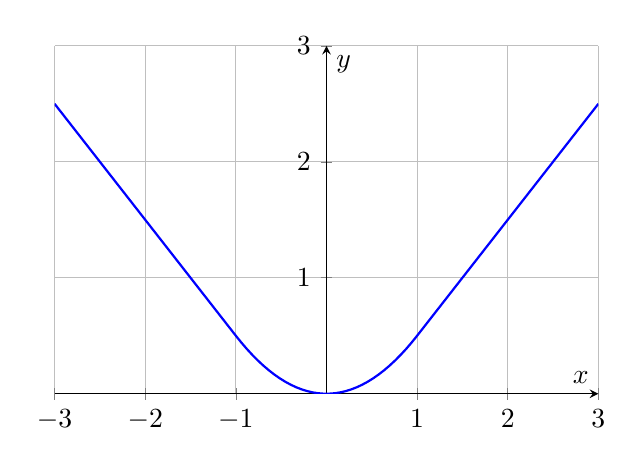
\begin{tikzpicture}
        \begin{axis}[
            title={},
            xlabel={$x$},
            ylabel={$y$},
            grid=major,
            domain=-3:3, % Bereich der x-Achse
            samples=100, % Anzahl der Punkte
            axis lines=middle, % Achsen durch die Mitte
            %xmin=-3, xmax=3, % Zoom Bereich auf der x-Achse
            width=0.7\textwidth, % Breitere Grafik
            height=6cm, % Schmalere Höhe der Grafik
            ymin=0.0, ymax=3, % Zoom Bereich auf der y-Achse
        ]
            % SmoothL1-Funktion
            \addplot[
                blue, 
                thick
            %]{abs(x) < 0.005 ? 0.5 * (x^2) / 0.005 : abs(x) - 0.5 * 0.005};
            ]{(abs(x) < 1) * (0.5 * x^2) + (abs(x) >= 1) * (abs(x) - 0.5)};
        \end{axis}
    \end{tikzpicture}
    \caption{$SmoothL1$ Loss Function}
    \label{fig:smoothL1}
\end{figure}
